\documentclass[11pt]{article}

\usepackage{hyperref}
\usepackage{amsmath}
\usepackage{enumerate}
\usepackage{tikz}
\usepackage{verbatim}
\usetikzlibrary{arrows}
\usetikzlibrary{positioning}
\newcommand{\bigO}{\ensuremath{\mathcal{O}}}

\title{\textbf{Algoritmen en Complexiteit HW 4}}
\author{Jelte Fennema (10183159)\\
		Jaap Koetsier (10440615)\\
        Abe Wiersma (10433120)}
\date{6 maart 2014}

\begin{document}

\maketitle

\begin{enumerate}
    \item
        \begin{enumerate}
            \item
                Dit is de begin graaf zonder stroomvergrotende paden:\\
                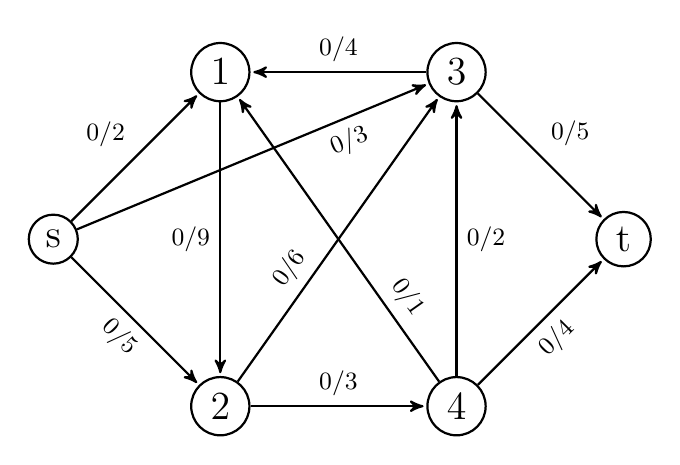
\begin{tikzpicture}[->,>=stealth',shorten >=1pt,auto,node distance=3cm,
                                    thick,main node/.style={circle,draw,font=\Large}]
                \node[main node] (S) {s};
                \node[main node] (1) [above right of=S] {1};
                \node[main node] (2) [below right of=S] {2};
                \node[main node] (3) [right of=1] {3};
                \node[main node] (4) [right of=2] {4};
                \node[main node] (T) [below right of=3] {t};
                \path[every node/.style={font=\small}]
                    (S)
                    edge node {0/2} (1)
                    edge node [below, sloped, pos=0.75]{0/3} (3)
                    edge node [below, sloped]{0/5} (2)

                    (1)
                    edge node [left] {0/9} (2)

                    (2)
                    edge node [sloped, pos=0.35] {0/6} (3)
                    edge node {0/3} (4)

                    (3)
                    edge node [above] {0/4} (1)
                    edge node {0/5} (T)

                    (4)
                    edge node [right] {0/2} (3)
                    edge node [below, sloped]{0/4} (T)
                    edge node [above, sloped, pos=.25] {0/1} (1);
                \end{tikzpicture}
                \\
                Om stroomvergrotende paden te vinden gebruiken we Dijkstra om
                het kortste pad qua aantal kanten te vinden. Een geheel gevulde
                kant wordt niet meer als kant gerekent.

                Het eerst gevonden stroomvergrotende pad is s, 3, t:

                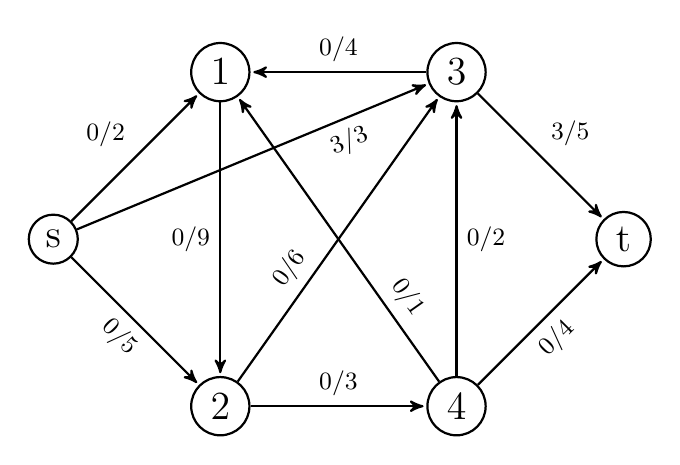
\begin{tikzpicture}[->,>=stealth',shorten >=1pt,auto,node distance=3cm,
                                    thick,main node/.style={circle,draw,font=\Large}]
                \node[main node] (S) {s};
                \node[main node] (1) [above right of=S] {1};
                \node[main node] (2) [below right of=S] {2};
                \node[main node] (3) [right of=1] {3};
                \node[main node] (4) [right of=2] {4};
                \node[main node] (T) [below right of=3] {t};
                \path[every node/.style={font=\small}]
                    (S)
                    edge node {0/2} (1)
                    edge node [below, sloped, pos=0.75]{3/3} (3)
                    edge node [below, sloped]{0/5} (2)

                    (1)
                    edge node [left] {0/9} (2)

                    (2)
                    edge node [sloped, pos=0.35] {0/6} (3)
                    edge node {0/3} (4)

                    (3)
                    edge node [above] {0/4} (1)
                    edge node {3/5} (T)

                    (4)
                    edge node [right] {0/2} (3)
                    edge node [below, sloped]{0/4} (T)
                    edge node [above, sloped, pos=.25] {0/1} (1);
                \end{tikzpicture}
                \\

                Het eerst volgende gevonden stroomvergrotende pad is s, 2, 4,
                t:\\

                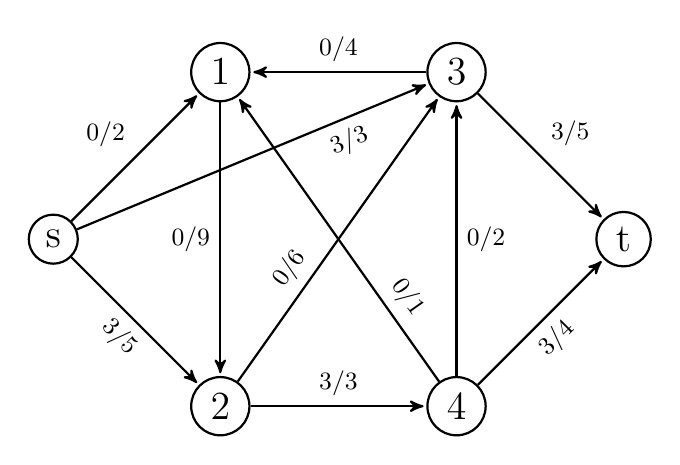
\begin{tikzpicture}[->,>=stealth',shorten >=1pt,auto,node distance=3cm,
                                    thick,main node/.style={circle,draw,font=\Large}]
                \node[main node] (S) {s};
                \node[main node] (1) [above right of=S] {1};
                \node[main node] (2) [below right of=S] {2};
                \node[main node] (3) [right of=1] {3};
                \node[main node] (4) [right of=2] {4};
                \node[main node] (T) [below right of=3] {t};
                \path[every node/.style={font=\small}]
                    (S)
                    edge node {0/2} (1)
                    edge node [below, sloped, pos=0.75]{3/3} (3)
                    edge node [below, sloped]{3/5} (2)

                    (1)
                    edge node [left] {0/9} (2)

                    (2)
                    edge node [sloped, pos=0.35] {0/6} (3)
                    edge node {3/3} (4)

                    (3)
                    edge node [above] {0/4} (1)
                    edge node {3/5} (T)

                    (4)
                    edge node [right] {0/2} (3)
                    edge node [below, sloped]{3/4} (T)
                    edge node [above, sloped, pos=.25] {0/1} (1);
                \end{tikzpicture}
                \\

                Het laatste gevonden stroomvergrotende pad is s, 2, 3, t:\\

                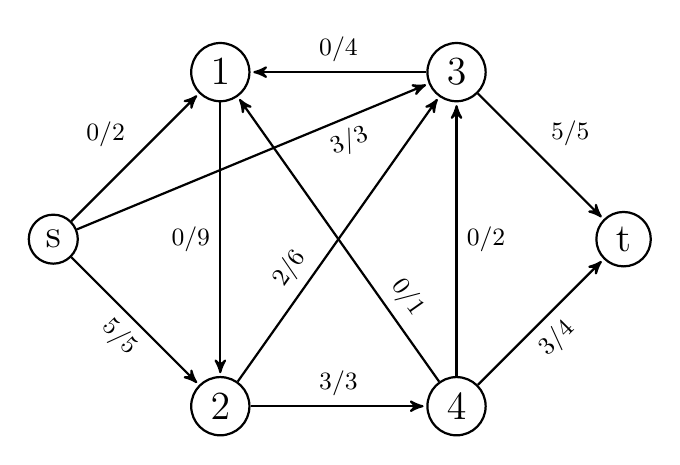
\begin{tikzpicture}[->,>=stealth',shorten >=1pt,auto,node distance=3cm,
                                    thick,main node/.style={circle,draw,font=\Large}]
                    \node[main node] (S) {s};
                    \node[main node] (1) [above right of=S] {1};
                    \node[main node] (2) [below right of=S] {2};
                    \node[main node] (3) [right of=1] {3};
                    \node[main node] (4) [right of=2] {4};
                    \node[main node] (T) [below right of=3] {t};
                    \path[every node/.style={font=\small}]
                        (S)
                        edge node {0/2} (1)
                        edge node [below, sloped, pos=0.75]{3/3} (3)
                        edge node [below, sloped]{5/5} (2)

                        (1)
                        edge node [left] {0/9} (2)

                        (2)
                        edge node [sloped, pos=0.35] {2/6} (3)
                        edge node {3/3} (4)

                        (3)
                        edge node [above] {0/4} (1)
                        edge node {5/5} (T)

                        (4)
                        edge node [right] {0/2} (3)
                        edge node [below, sloped]{3/4} (T)
                        edge node [above, sloped, pos=.25] {0/1} (1);
                \end{tikzpicture}
                \\

                De maximale stroom is dus 8, want dat gaat s uit en gaat t in.

            \item
                Het gelaagde netwerk:\\
                \def\layersep{2.5cm}
                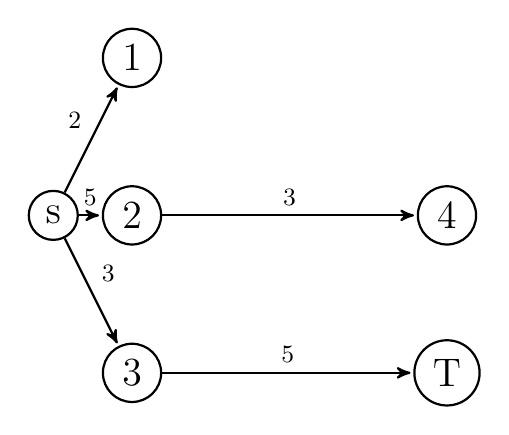
\begin{tikzpicture}[->,>=stealth',shorten >=1pt,auto,node distance=3cm,
                                    thick,main node/.style={circle,draw,font=\Large}]
                    \node[main node] (S) {s};
                    \node[main node] (1) at (\layersep, 2cm) {1};
                    \node[main node] (2) at (\layersep, 0cm) {2};
                    \node[main node] (3) at (\layersep, -2cm) {3};
                    \node[main node] (4) at (5cm, 0cm) {4};
                    \node[main node] (T) at (5cm, -2cm) {T};
                    \path[every node/.style={font=\small}]
                        (S)
                        edge node {2} (1)
                        edge node {3} (3)
                        edge node {5} (2)

                        (2)
                        edge node {3} (4)

                        (3)
                        edge node {5} (T)
                        ;
                \end{tikzpicture}


            \item
                Links is s, 1, 2, 3 en rechts 4, t. De minimale capaciteit van
                de die cut is dan 8, dit is hetzelfde als de maximale flow die
                gevonden is in 1c.

        \end{enumerate}

    \item
        Dit probleem is uit te drukken als een netwerk waarin de verschillende kabels
        en frequenties nodes zijn.

        Van R lopen kanten naar de kabel nodes. De kant vanuit R naar de node
        van kabel $j$ heeft een capaciteit van $n_j$. Vanuit elke kabel node
        lopen kanten naar elke frequentie node. Deze kanten hebben allemaal een
        capaciteit van $1$. Vanuit elke frequentienode loopt dan weer een kant
        naar S. De capaciteit voor deze kant voor elke frequentie $f$ is het
        aantal keer $n$ dat $f$ voorkomt in $C$.


    \item
        \begin{enumerate}
            \item

            \item

            \item

        \end{enumerate}

    \item

\end{enumerate}

\end{document}
